\documentclass{beamer}

\usepackage{fontspec,xunicode,xltxtra}

\XeTeXlinebreaklocale "zh"
\XeTeXlinebreakskip = 0pt plus 1pt minus 0.1pt

%\setmainfont[Mapping=tex-text]{AR PL UMing CN:style=Light}
%\setmainfont[Mapping=tex-text]{AR PL UKai CN:style=Book}
%\setmainfont[Mapping=tex-text]{WenQuanYi Zen Hei:style=Regular}
%\setmainfont[Mapping=tex-text]{WenQuanYi Zen Hei Sharp:style=Regular}
%\setmainfont[Mapping=tex-text]{AR PL KaitiM GB:style=Regular} 
%\setmainfont[Mapping=tex-text]{AR PL SungtiL GB:style=Regular} 
%\setmainfont[Mapping=tex-text]{WenQuanYi Zen Hei Mono:style=Regular} 

\newfontfamily\hei{WenQuanYi Micro Hei}
\newfontfamily\whei{WenQuanYi Zen Hei}
\newfontfamily\kai{AR PL UKai CN}
\newfontfamily\song{AR PL UMing CN}
\newfontfamily\bhei{cwTeXHeiBold}
\setmainfont[Mapping=tex-text]{WenQuanYi Micro Hei}
\setsansfont[Mapping=tex-text]{AR PL UKai CN}
\setmonofont[Mapping=tex-text]{WenQuanYi Zen Hei Mono}
\renewcommand{\baselinestretch}{1.25}


\mode<presentation>
{
   \usetheme{Warsaw}
  % or ...
 % \usetheme{default}

  \setbeamercovered{transparent}
  % or whatever (possibly just delete it)
}


\usepackage[english]{babel}
% or whatever
\usepackage{tikz}
\usepackage{pgflibraryarrows}
\usepackage{pgflibrarysnakes}
\usepackage{subfig}
\usepackage{xcolor}
\usepackage{multirow}
\usepackage{listings}
\usepackage{pgfpages}
\usepackage{eso-pic} 
\usepackage{animate}  
\usepackage{media9}
% or whatever

\title[GAI] % (optional, use only with long paper titles)
{生成式AI工具在应用数学教学辅助中的探索}

%\subtitle
%{Scientific Computing} % (optional)

\author[Wang HY] % (optional, use only with lots of authors)
{王何宇}
% - Use the \inst{?} command only if the authors have different
%   affiliation.

\institute[ZJU] % (optional, but mostly needed)
{
浙江大学数学科学学院
}
% - Use the \inst command only if there are several affiliations.
% - Keep it simple, no one is interested in your street address.

\date[Short Occasion] % (optional)
{2024 年 6 月, 浙江大学, 杭州}


% If you have a file called "university-logo-filename.xxx", where xxx
% is a graphic format that can be processed by latex or pdflatex,
% resp., then you can add a logo as follows:

\pgfdeclareimage[height=1cm]{university-logo}{images/zju.jpg}
\logo{\pgfuseimage{university-logo}}

% Delete this, if you do not want the table of contents to pop up at
% the beginning of each subsection:
%\AtBeginSubsection[]
%{
%  \begin{frame}<beamer>{Outline}
%    \tableofcontents[currentsection,currentsubsection]
%  \end{frame}
%}


% If you wish to uncover everything in a step-wise fashion, uncomment
% the following command: 

%\beamerdefaultoverlayspecification{<+->}

% for movie play in pdfpc
%\setbeamertemplate{navigation symbols}{} % don't use navigation tools on slides

% use our .sty file for simple movie commands
%\usepackage{pdfpc-commands}


\begin{document}

\begin{frame}
 \titlepage
\end{frame}
\begin{frame}{Outline}
  \tableofcontents
  % You might wish to add the option [pausesections]
\end{frame}

\section{背景:培养目标和课程}
\begin{frame}
\frametitle{应用数学学科的培养目标}
参考2024年浙江大学信息与计算科学专业培养方案:
\begin{itemize}
\item 2. 具有扎实的数学基础,精通应用与计算数学的基本理论和常用方法;
\item 4. 具备解决实际问题的卓越能力,包括数学建模能力、数值算法设计能力、程序编制和软件开发能力,并善于运用这些能力解决实际问题。  
\end{itemize}
\begin{figure}
    \centering 

\includegraphics[width=0.3\textwidth]{images/MATH.jpg}

\includegraphics[width=0.1\textwidth]{images/plus.jpg}

\includegraphics[width=0.3\textwidth]{images/COMPUTER.jpg}
\end{figure}
\end{frame}

\begin{frame}
    \frametitle{课程《数学软件》简介} 
\begin{itemize}
    \item<1-> 开设对象:数学科学学院信息与计算专业和强基班一年级本科生
    \item<1-> 开始时间:第一学年第二学期,共 16 周
    \item<1-> 主要目标:掌握进一步学习所必须的计算机技能和编程能力。
    \item<2-> 具体要求:
        \begin{enumerate} \tiny
            \item 科技文献查阅;
            \item 科技文档写作;
            \item 在 Linux 操作系统上进行基本科研和学习的概念和技能基础;
            \item 利用开源社区进行编程和软件开发工作的概念和技能基础;
            \item 主要数学软件和开源库;
            \item 和应用数学科研相关的计算机技术,如并行计算和计算可视化等等。
            \item ...
        \end{enumerate}
\end{itemize}    
\end{frame}

\begin{frame}
    \frametitle{实际困难和矛盾}
    \begin{itemize}
        \item 宽泛的课程内容和数学院学生紧张的专业学习;
        \item 技术性内容的枯燥和数学院学生兴趣驱动的学习模式;
        \item 基于数学建模的顶层设计需求和繁琐的技术细节处理;
    \end{itemize}
    \begin{figure}
        \centering 
    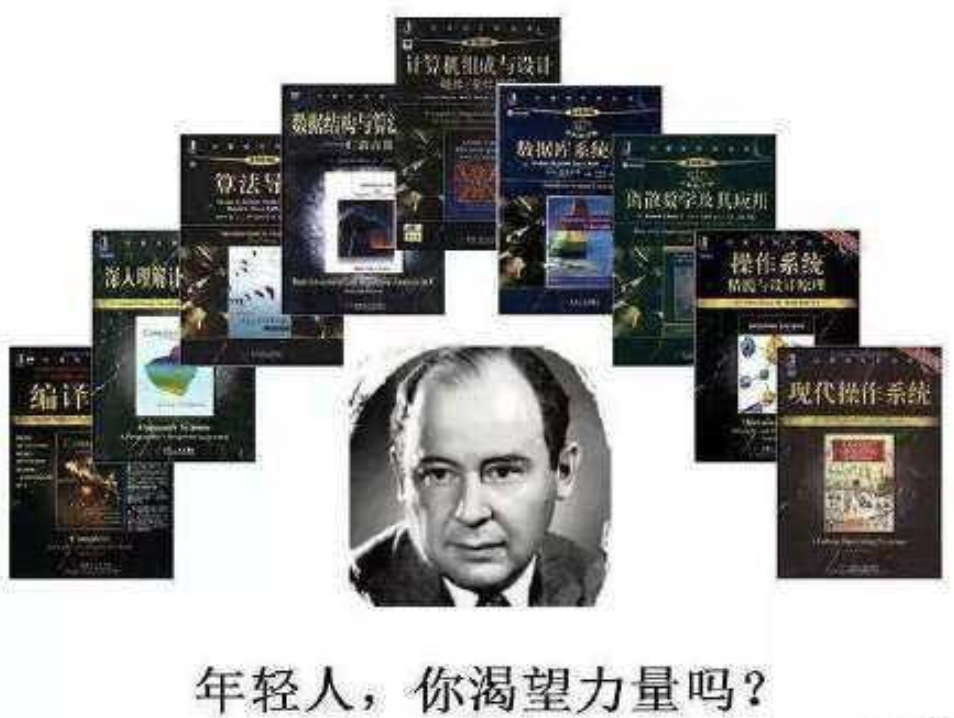
\includegraphics[width=0.3\textwidth]{images/computerbook.png}
    
\includegraphics[width=0.1\textwidth]{images/x.png}
    
\includegraphics[width=0.3\textwidth]{images/hard.png}
    \end{figure}    
    \begin{itemize}
        \item<2-> 教师和助教往往沉溺于技术细节的答疑,无法做更多的教学设计和指导;
    \end{itemize}
\end{frame}

\begin{frame}
    \frametitle{生成式 AI 工具带来的转机}
    \begin{figure}
        \centering
        
\includegraphics[width=0.75\textwidth]{images/ChatMate.png}
    \end{figure}
    \begin{itemize}
        \item 浙江大学计算机科学与技术学院{\hei 陈为教授}团队提供了一种基于生成式 AI 技术的智能助教平台 {\hei ChatMate};
    \end{itemize}
\end{frame}

\section{教学案例:Conway 的生命游戏}

\begin{frame}
    \frametitle{教学案例的选择原则}
    \begin{itemize} \small
        \item 和后续学习有关,但不需要太多基础数学知识就能够理解;
        \item 有一定的趣味性。和计算机技术有关,能形成一个需要一定技术支持的小项目。
        \item 我们使用过的案例有 Manderbrot 集合、Conway 生命游戏、三体可视化、伪随机数生成和检测等等。
        \item 数学学习本身不是主要目的,围绕这些主题的计算机技术的熟练才是。我们下面选择 Conway 生命游戏作为案例。
    \end{itemize}
    \begin{center}
    \includemedia[  
        width=0.3\textwidth,  
        height=0.3\textwidth,  
        activate=pageopen,  
        addresource=movie/output.mp4,  
        flashvars={  
           source=movie/output.mp4  
          &autoPlay=true  
          &loop=true  
        }
      ]{}{VPlayer.swf}  
    \end{center}
\end{frame}

\begin{frame}
    \frametitle{预习阶段:自主文献查阅和调查报告撰写}
    \begin{itemize}
        \item<1-> 这个案例实际发生在第三周,通过前序学习,学生应该已经基本掌握:
            \begin{enumerate} \small
                \item 结合 ChatMate 工具和搜索引擎进行文献查阅;
                \item 用 latex 撰写科技文档,并用 bibtex 管理文献;
            \end{enumerate}
        \item<1-> 学生需要在 ChatMate 的帮助下撰写一份调查报告,介绍 Conway 生命游戏的历史、基本规则和实现;
        \item<2-> 重点:进一步熟练科技文档查阅、撰写和管理的技能。\textcolor{red}{生成式 AI 给出的文献线索并不一定可靠!} 
        \item<3-> 强调:对文献的正确性验证是作者的责任,合理使用 AI 工具并不意味着盲从。
    \end{itemize}
\end{frame}

\begin{frame}
    \frametitle{授课阶段:实现 Conway 生命游戏的可视化}
    \begin{itemize}
        \item 生命游戏的迷人之处在于其简单的规则和复杂的演化过程;
        \item 用生命游戏做诱饵,在 ChatMate 的帮助下,通过课堂演示和提示,让学生逐步实现这个项目。激发学习计算机技术,探索数学问题的兴趣。
        \item 教师将任务做适当的分解,使得正好每一步都能够用 ChatMate 的帮助下完成。并用课堂演示让学生觉得``这并不困难''。
        \item \textcolor{red}{根本目的:引导学生在实际工作中学习计算机技术和编程。} 而 AI 工具使得这一目的成为可能。
        % 比如这个案例的主要难点在动态可视化和 RLE 格式文件的自动解码。教师将这两个部分独立出来并形成解决步骤,让学生在 AI 工具的辅助下自行解决。
        % \item 生命游戏的迷人之处在于其简单的规则和复杂的演化过程;但这一点要用 C 语言实现并不容易。特别是当大部分学生根本没有学过 C 语言时。
        % \item 用生命游戏做诱饵,在 ChatMate 的帮助下,通过课堂演示和提示,让学生逐步实现这个项目,并在这个过程中,激发学习计算机技术,探索数学问题的兴趣。
        % \item 教师将任务做适当的分解,使得正好每一步都能够用 ChatMate 的帮助完成。并用丝滑的操作让学生觉得``这并不困难''。
        % 比如这个案例的主要难点在动态可视化和 RLE 格式文件的自动解码。教师将这两个部分独立出来并形成解决步骤,让学生在 AI 工具的辅助下自行解决。
    \end{itemize}
    \begin{figure}
        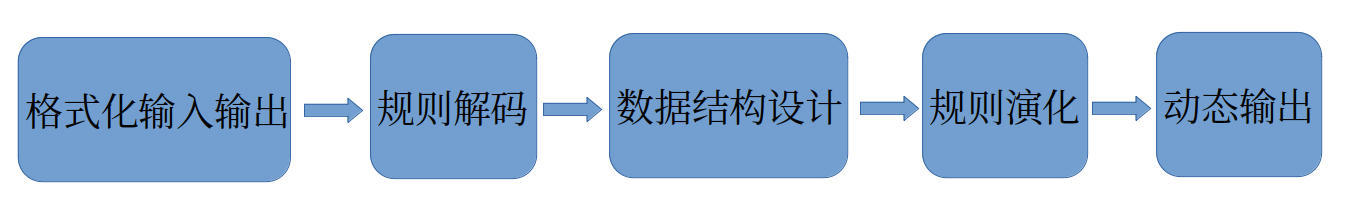
\includegraphics[width=0.75\textwidth]{images/steps.png}
    \end{figure}
\end{frame}

\begin{frame}
    \frametitle{作业阶段:学生独立完成项目}
    \begin{itemize}
        \item<1-> 学生个人形成完整的代码和报告,并以项目管理工具 git 进行提交,由助教和教师评阅。
        \item<1-> 鼓励学生在 ChatMate 的帮助下,自行解决遇到的问题。教师和助教只在必要时给予提示。
        \item<1-> 鼓励学生在作业之外,进一步探索生命游戏的变种和相关的数学问题,并编程验证和实现。
        \item<2-> \textcolor{red}{重点:AI 可以很好的解决基础编程错误和技术细节,但无法解决较为复杂的逻辑。让学生反思人和 AI 的关系。}
    \end{itemize}    
\end{frame}

\begin{frame}
    \frametitle{案例目的:练习和编程}
    \begin{itemize}
        \item 练习文献查阅、管理、撰写的技能;
        \item 初步掌握 C 语言的基本语法和格式化输入输出,文件操作。并通过项目熟练;
        \item 进一步体会 AI 的作用和 AI 的边界。
        \item 最终效果:大部分同学在这一周能够初步实现生命游戏的可视化,并对 C 语言有一定的了解。这将在未来提升他们进一步掌握底层编程技术的信心。
        % https://git.zju.edu.cn/3230102179/math-soft.git
    \end{itemize}    
\end{frame}

\section{总结和反思}

\begin{frame}
    \frametitle{总结和反思}
    \begin{itemize}
        \item<1-> 正确使用 AI 对未来的科技工作者而言是必须掌握的技能;
        \item<1-> 生成式 AI 工具在教学辅助中的确实能通过对基本概念,技术文档和科技文档的实时答疑,极大提升学生学习效率和信心;
        \item<2-> 隐忧:如果学生在 AI 帮助下掌握了某项技能,他是否会形成依赖?如果是,能否认为他真正地掌握了这项技能?
        % 回答一:对编程这样的技能,用更多更复杂的项目例子去锻炼学生,让他们通过反复锻炼,逐渐形成自己的坚实技能体系。优秀的学生,甚至可以更早参与到实际科研中,进一步得到真正的锻炼。
        % 回答二:也许不用太担心这个问题。这就好比我是做计算数学的,如果没有计算机,我还会不会数学?可能我的数学水平会不足以做理论数学研究,但这个问题的前提不存在。AI 就像计算机一样,已经无法和人类社会的发展脱离了。
        \item<3-> AI 的快速发展和广泛应用,也给教育工作者带来了新的挑战和机遇;
    \end{itemize}
\end{frame}

\begin{frame}
    \begin{center}
        \Huge \textcolor{red}{谢谢!}
    \end{center}
\end{frame}

\end{document}